\documentclass[10pt,twocolumn]{article}
\usepackage[letterpaper,margin=0.68in,columnsep=0.25in]{geometry}
\usepackage[T1]{fontenc}
\usepackage[utf8]{inputenc}
\usepackage{times}
\usepackage{microtype,graphicx,booktabs,amsmath,amssymb,tabularx}
\usepackage[hidelinks]{hyperref}
\setlength{\parskip}{0pt}
\newcolumntype{Y}{>{\raggedright\arraybackslash}X}
\renewcommand{\paragraph}[1]{\smallskip\noindent\textbf{#1}\;}

\title{\vspace{-1.6em}\textbf{Agentic Neural Audio Synthesis: A Skill for LLM Agents\\to Disentangle and Play Frozen Neural Audio Codecs}\vspace{-0.6em}}
\author{Moisés Horta Valenzuela\\ \small SEMILLA.AI Studio \quad \href{https://semilla.ai}{\texttt{https://semilla.ai}}}
\date{\vspace{-1.8em}}
\usepackage{caption}
\makeatletter
\g@addto@macro\@maketitle{%
  \vspace{-0.6em}%
  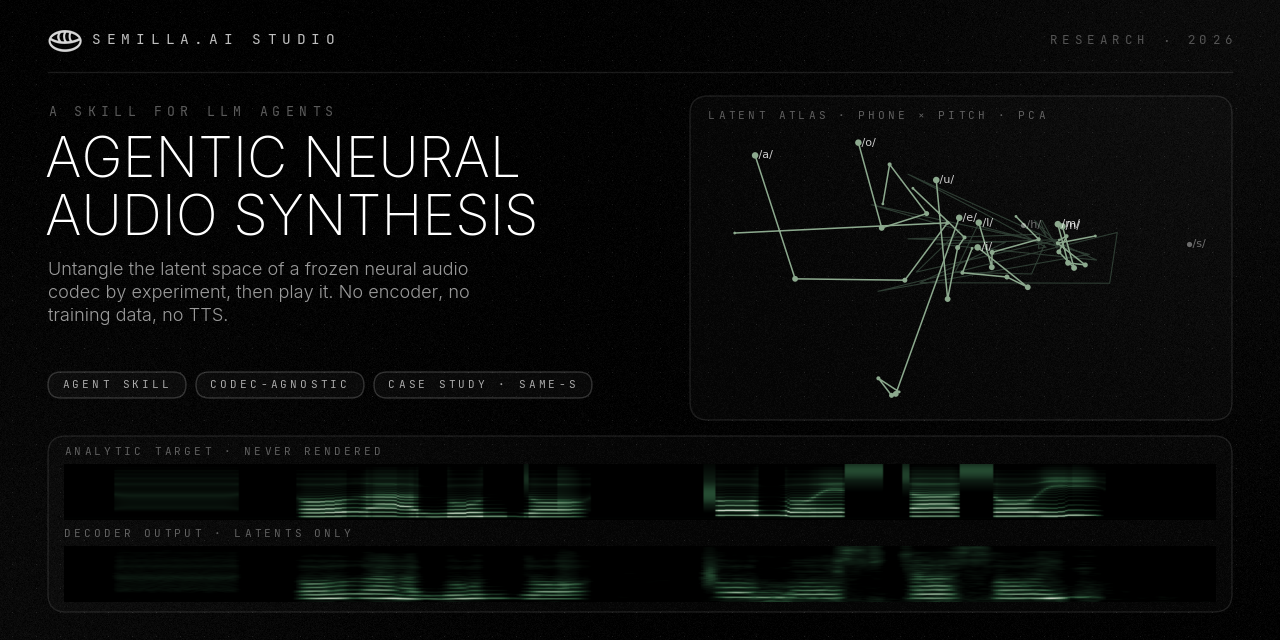
\includegraphics[width=\textwidth]{fig_banner.png}\par\vspace{-0.3em}%
  \captionof{figure}{Agentic Neural Audio Synthesis. Right: the latent atlas an LLM agent mapped for the case study's female voice. Phone\,$\times$\,pitch ladders (165--320\,Hz; larger dots are higher pitch) are projected on the atlas's first two principal components, with the decoded sentence drawn as a path. Bottom: the analytic target, never rendered to audio, and the frozen decoder's output for the final take of ``hola mundo, cómo estás hoy?'' (log-mel).}\label{fig:banner}%
  \vspace{0.6em}}
\makeatother

\begin{document}
\maketitle

\begin{abstract}
Pretrained neural audio codecs contain powerful decoders, but their latent spaces are undocumented and entangled. Generating with them normally requires an encoder, a learned prior and training data. We introduce \emph{Agentic Neural Audio Synthesis} (ANAS), in which an LLM agent with code execution disentangles the latent space of a frozen decoder by experiment. It then uses that map to synthesise sounds requested in natural language, with no encoder, no audio data and no ability to listen. We package the method as a codec-agnostic \emph{skill}: a natural-language procedure, plus reference code, that an agent loads on demand. We distilled the skill from an autonomous session in which an LLM agent mapped a Stable Audio--family codec. The agent found four things: pitch is not a shared latent direction (mean $|\cos|$ 0.09--0.12 between per-unit pitch directions); latent frames are exactly local within 6-frame windows; the loss landscape needs noise smoothing; and the decoder games periodicity objectives with a patch-repetition buzz. Applied to making the codec speak a Spanish sentence, the procedure raised median harmonics-to-noise ratio from $-6.5$ to $17.9$\,dB and vowel identification from 10\,\% to 90--100\,\% over 23 logged iterations. We release the skill, the code and the full log.
\end{abstract}

\section{Introduction}
Neural audio codecs \cite{zeghidour2021soundstream,defossez2022encodec,kumar2023dac} and latent-diffusion autoencoders \cite{evans2024fast} compress audio into short sequences of latents from which a decoder reconstructs high-fidelity sound. Generation is normally delegated to a learned prior trained on large corpora \cite{borsos2023audiolm,evans2024fast}. The decoder alone is a general-purpose instrument: every latent sequence produces \emph{some} sound. Its latent space, however, is learned, entangled and undocumented, so playing it directly requires knowing where sounds live and how they combine.

We ask whether an LLM agent can find this out by itself and then use what it found to produce new sounds on request. The agent does not emit audio tokens. It writes programs: it reads the decoder, probes it, writes physics-based targets from its own domain knowledge, optimises latents by gradient descent, measures the result with proxies (it cannot hear), and revises the method when something fails. Our answer is a reusable \emph{skill} that encodes this process for any agent and any codec.

\paragraph{Contributions.} (1)~The ANAS problem: decoder-only, data-free, agent-driven synthesis from a natural-language request. (2)~A codec-agnostic skill of eight phases (Table~\ref{tab:skill}). Each phase says what it reveals about the latent space and how to test that on a new codec. (3)~Findings about a real codec's latent space, uncovered autonomously by the agent. (4)~A case study with a complete 23-iteration record, released with the skill and reference code.

\begin{figure*}[t]
\centering
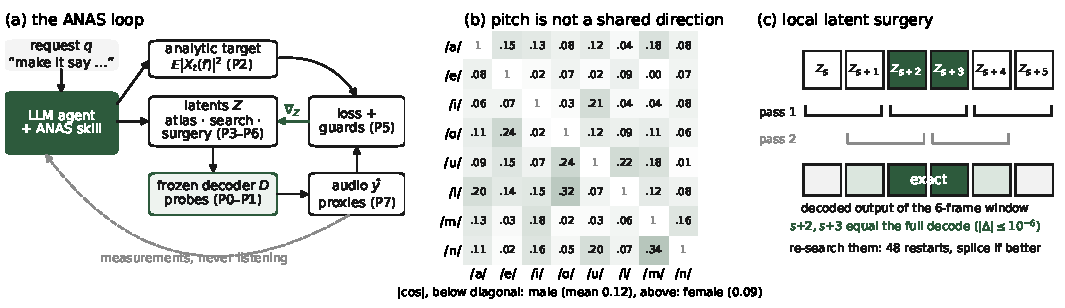
\includegraphics[width=\textwidth]{fig_schematic.pdf}
\vspace{-1.6em}
\caption{(a)~The ANAS loop. Guided by the skill, the agent writes an analytic target and the latents. The frozen decoder renders audio, a spectral loss with guards returns gradients to the latents, and perceptual proxies return measurements to the agent, which never listens. There is no encoder, no data and no TTS. Phase labels refer to Table~\ref{tab:skill}. (b)~A disentanglement diagnostic from the case study: $|\cos|$ between per-phone pitch directions (slope of the latent on $\log F_0$) for the male (below the diagonal) and female (above) atlases. Near-orthogonal directions mean pitch is entangled with phone identity, so the atlas must be a unit\,$\times$\,pitch grid. (c)~Why local surgery is exact. The decoder attends within 2-frame chunks in one pass and within chunks shifted by one frame in a second pass, so decoding a 6-frame window that starts at an even frame $s$ reproduces the full-context output of frames $s{+}2$ and $s{+}3$ (measured $|\Delta|\le10^{-6}$). Only those two frames are re-searched.}
\label{fig:schematic}
\vspace{-0.9em}
\end{figure*}

\section{Related work}
\paragraph{LLM agents for audio.} WavJourney \cite{liu2025wavjourney}, AudioGPT \cite{huang2024audiogpt}, MusicAgent \cite{yu2023musicagent}, WavCraft \cite{liang2024wavcraft} and Audio-Agent \cite{wang2024audioagent} use an LLM to plan and call pretrained generators (TTS, text-to-audio, music models) and editing tools. The LLM never touches a latent space, and quality is bounded by the tools. ANAS forbids such tools: the only sound source is a frozen decoder without a prior.

\paragraph{Optimising through frozen generators.} VQGAN-CLIP \cite{crowson2022vqganclip} optimises a frozen image decoder's latents against a CLIP score. DITTO \cite{novack2024ditto} optimises the initial noise of a text-to-music diffusion model against differentiable feature losses. CTAG \cite{cherep2024ctag} searches synthesizer parameters to maximise CLAP similarity, sound-matching work compares losses for iterative parameter search \cite{salimi2025soundmatching}, and LVNS-RAVE \cite{guo2024lvnsrave} runs novelty search in the latent space of RAVE \cite{caillon2021rave}. All of these fix the objective and the search algorithm in advance and rely on a learned prior or critic. In ANAS the agent writes the objective from domain knowledge, discovers how the decoder fails, and redesigns both objective and search.

\paragraph{Interpreting codec latents.} Disentanglement is usually imposed during training \cite{higgins2017beta} or found post hoc by linear analysis \cite{harkonen2020ganspace}. For audio codecs, probing and attribute prediction show that pitch, content and speaker are entangled in codec tokens \cite{sadok2025interpretability}, and sparse autoencoders recover interpretable features from audio latents \cite{paek2025sae}. These methods need recorded or labelled audio. Our agent maps structure by synthesis experiments alone, and reaches a compatible conclusion: pitch is not a shared direction.

\paragraph{Agents as experimenters, and skills.} MAIA \cite{shaham2024maia} runs experiments on vision models to explain their units. FunSearch \cite{romera2024funsearch} and AlphaEvolve \cite{novikov2025alphaevolve} evolve programs against automatic evaluators. The AI Scientist \cite{lu2024aiscientist} automates the ML research loop. Voyager \cite{wang2023voyager} stores what an agent learns as a library of executable skills. Agent Skills package procedures as files that agents load on demand \cite{xu2026agentskills}, and recent work distils expert knowledge into such skills \cite{zhou2026colleague} and tests what transfers \cite{kassis2026mimeo}. ANAS distils an agent's own successful research trajectory into a skill for other agents. To our knowledge, no prior work has an LLM agent map a frozen neural audio decoder by experiment and then synthesise requested sounds from it without a prior, data or an encoder.

\section{Problem setting}
Let $D:\mathbb{R}^{d\times T}\!\to\!\mathbb{R}^{c\times hT}$ be a frozen, differentiable decoder with latent width $d$, hop $h$ and $c$ channels. Given a request $q$, an agent with a code interpreter, the decoder file and numerical libraries must return $Z$ such that $D(Z)$ realises $q$. Four constraints apply. Audio may come only from $D$. The encoder is never called. No recordings, datasets or TTS may be used. The agent cannot listen. Domain knowledge enters only through targets and proxies. ANAS differs from inversion \cite{xia2022gan} because there is no example to invert, and from DDSP \cite{engel2020ddsp} because the decoder is the only sound source. For quantised codecs, the agent optimises the continuous embedding that the decoder consumes.

\begin{table*}[t]
\centering\footnotesize
\setlength{\tabcolsep}{3.5pt}
\begin{tabularx}{\textwidth}{@{}>{\raggedright\arraybackslash}p{2.1cm}YYY@{}}
\toprule
phase & agent action (codec-agnostic) & what it reveals about the latent space & finding on SAME-S (case study) \\
\midrule
P0 reconnaissance & read the decoder source; measure the receptive field by perturbing one frame & rate, hop, width, normalisation, frame constraints, temporal locality & 44.1\,kHz, $d{=}256$, $h{=}4096$; chunked attention $\Rightarrow$ $\pm$1-frame receptive field; even $T$ \\
P1 anchors \& probes & decode zero, random and static latents; find a silence latent by energy minimisation; per-dimension sweeps; input-projection SVD & where silence, noise and tone live; whether the code is distributed & zeros $\neq$ silence ($-34$\,dB); static latent $\to$ pitched buzz; silence latent at $-65$\,dB; all 256 dims used, single dims barely matter \\
P2 target as physics & write the request as parameter tracks and compute its expected STFT power in closed form (Eq.~\ref{eq:target}) & nothing yet; supplies a data-free reference & source--filter Spanish phonetics: formants, F0 contour, durations, room tone \\
P3 unit atlas & optimise one static latent per unit, then per unit $\times$ pitch; measure the factor geometry & which factors are shared directions and which are entangled & per-unit $\partial z/\partial\log F_0$ near-orthogonal (mean $|\cos|$ 0.12 male, 0.09 female) $\Rightarrow$ the atlas must be a grid; its PCA plane is phonetic \\
P4 composition \& search & interpolate the atlas; population + frame-wise crossover; latent noise $\sigma$ & how rough the landscape is; how independent frames are & $\sigma{=}0$ leaves a good solution (4.7$\to$9--19\,dB), $\sigma{=}0.1$ holds it; frame splicing nearly lossless \\
P5 guarded refinement & add perceptual-structure losses; after each, search for the decoder's cheat and guard it & the decoder's degenerate modes & octave-up; identical 256-sample patches $\Rightarrow$ 172.27\,Hz buzz ($=44100/256$), also hidden in fricative noise \\
P6 local surgery & measure the exact-window property; re-search a few frames with many restarts; splice & where global optimisation is stuck in local minima & a 6-frame window is exact for its 2 middle frames ($10^{-6}$); this fixes stop bursts and closures \\
P7 proxy evaluation & perceptual proxies, per-frame audit, rejection rule, numbered log & attractors that the plan should not fight & accent forced to 158\,Hz collapses; attractor at $\approx$139\,Hz $\Rightarrow$ branch rejected \\
\bottomrule
\end{tabularx}
\vspace{-0.5em}
\caption{The ANAS skill. Each phase is defined without reference to a specific codec. The last column shows what the agent found when it ran the procedure on the SAME-S decoder.}
\label{tab:skill}
\vspace{-0.9em}
\end{table*}

\section{The skill}
\label{sec:skill}
The skill (Table~\ref{tab:skill}, Fig.~\ref{fig:schematic}a) is a markdown procedure in the Agent Skills format \cite{xu2026agentskills}. Its metadata tells an agent when to load it. Its body gives phases, default values, known pitfalls and pointers to a reference implementation. Codec-specific constants such as hop, patch size and receptive field are \emph{discovered} in P0--P1, never assumed.

\paragraph{Analytic target (P2).} The request is written as parameter tracks: partial frequencies and amplitudes, resonances, noise level and band, envelopes. Their expected STFT power is evaluated in closed form:
\begin{equation}
\mathbb{E}|X_t(f)|^2=\textstyle\sum_k \tfrac{a_{tk}^2}{4}\,|W(f-f_{tk})|^2+\sigma_t^2\,S_t(f)\,\|w\|^2,
\label{eq:target}
\end{equation}
where $W$ is the window transform and $S_t$ a shaped noise spectrum. For speech, $f_{tk}=kF_{0,t}$ and $a_{tk}$ follows a cascade source--filter model \cite{fant1960acoustic,klatt1980software} with Spanish formants \cite{quilis1981fonetica}. For percussion, modal partials replace harmonics. The target is never rendered as audio.

\paragraph{Objective (P2--P5).} With $\hat y=D(Z+\sigma\epsilon)$, the base term is a multi-resolution \cite{yamamoto2020parallel} log-distance on the mel spectrum of the STFT \emph{magnitude}, $\mathcal{L}_{\text{mel}}=\frac{1}{|R|}\sum_r\overline{|20\log_{10}\frac{M_r(\hat y)+\varepsilon_r}{A_r+\varepsilon_r}|}$, plus the same on linear-frequency partials. A log-\emph{power} loss makes silence an attractor because its gradients vanish there. Structure losses use the normalised autocorrelation $\rho(\tau)$ at the planned period $P$, each paired with guards against the cheats found in P5:
\begin{align}
\mathcal{L}_{\text{per}}=\operatorname{mean}\big[&(0.97-\rho(P))_+ + (\rho(\tfrac{P}{2})-0.8)_+ \nonumber\\
&+\mathbf{1}_{|P-p|>25}\,(\rho(p)-0.85)_+\big],
\end{align}
with $p$ the decoder's output patch length, plus $(|\rho(p)|-0.1)_+$ on frames planned as noise and a silence guard. Here $\rho(P)=0.97$ corresponds to an HNR of about 15\,dB \cite{boersma1993accurate}. The general rule is that \emph{every new objective invites a new degenerate solution}, a form of specification gaming \cite{krakovna2020specification}, so P5 alternates objective and guard.

\paragraph{Search (P3--P6).} Atlas entries are static latents optimised with 6--12 restarts per unit in one batch. A sequence is initialised frame by frame as a time-overlap-weighted mix of entries interpolated in $\log F_0$. A population is optimised with Adam. Every 150 steps its best frames are spliced into an elite, which is valid because of the locality measured in P0. Latent noise $\sigma\in[0.05,0.1]$ smooths the landscape \cite{cohen2019certified}. In analysis-by-synthesis re-pitching \cite{bell1961reduction}, the target adopts the decoder's measured F0 within $\pm$3 semitones. Local surgery re-searches only the frames whose output a short window reproduces exactly (Fig.~\ref{fig:schematic}c): 48 restarts in one batch, spliced back if better.

\paragraph{Evaluation without hearing (P7).} Speech proxies: vowel identity from LPC formants, F0 error by pYIN \cite{mauch2014pyin}, voicing recall and false alarms, median HNR, pause depth, and a per-frame error audit at each consonant. Music proxies (onset timing, per-event spectra, decay times) are listed in the skill. Every iteration goes in a numbered folder with audio, latents and metrics, and dead ends stay in the log.

\section{Case study: making SAME-S speak}
\label{sec:case}
\paragraph{Setup.} SAME-S is a Stable Audio--family autoencoder shipped as TorchScript (Table~\ref{tab:skill}, P0). An LLM coding agent received one request: use only the decoder to produce ``hola mundo, cómo estás hoy?'' as realistically as possible. There was one human intervention, a switch to the GPU. The run took about 3.9\,h on one Apple M4~Max (MPS, fp32). The run made 170 tool calls. The skill's phases map onto the iteration log: 00 (P0--P1); 01--02 (loss failures); 02b, 04, 15 (atlas); 03, 05--07 (composition); 08--11, 20--21 (refinement); 12--14, 18--19 (surgery).


\begin{figure*}[t]
\centering
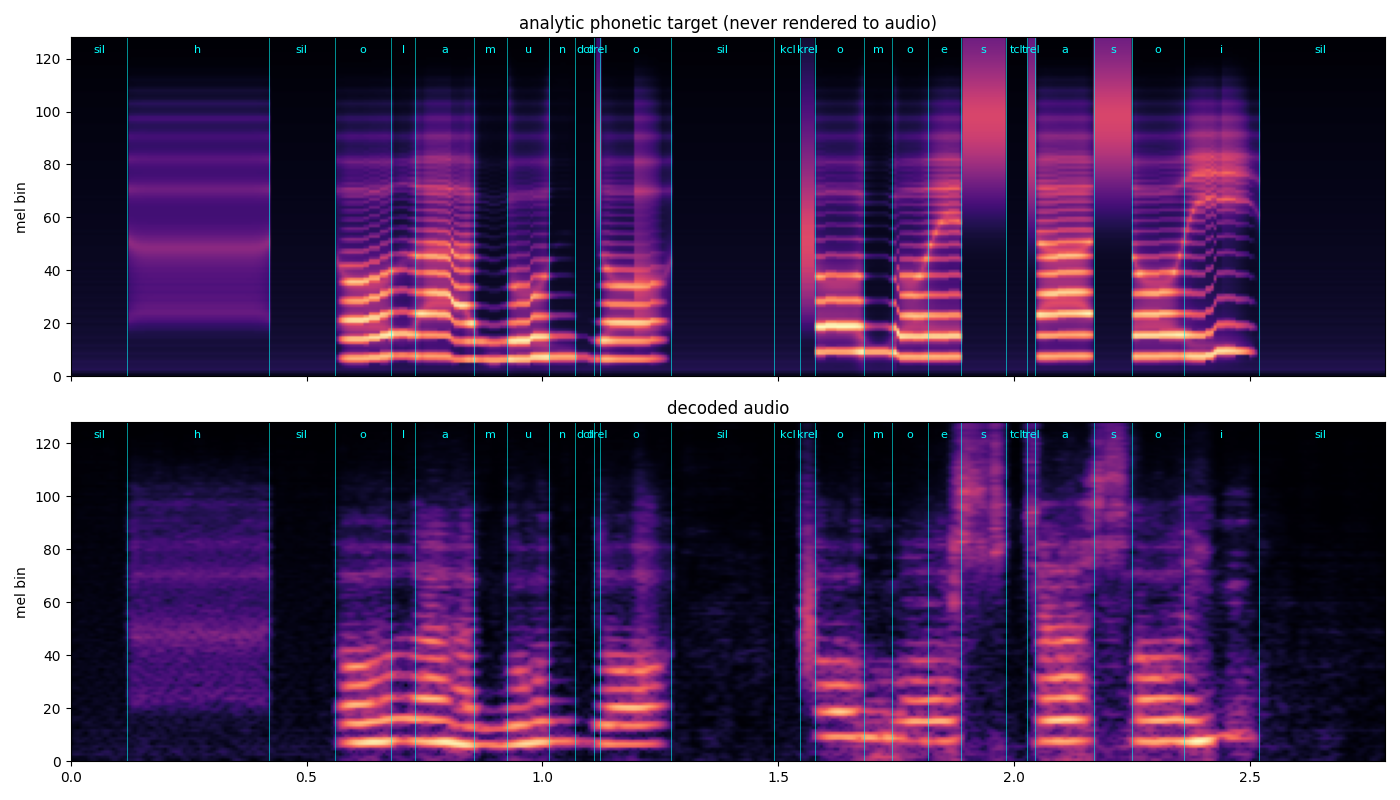
\includegraphics[width=\textwidth,height=0.22\textheight]{fig_target_vs_decoded.png}
\vspace{-1.8em}
\caption{Analytic target (top, never rendered to audio) and decoder output after iteration 20 (bottom) for the female take, including an inhale. Harmonics, formant transitions, the /k/ burst, the silent /t/ closure and both /s/ are reproduced.}
\label{fig:mel}
\vspace{-0.9em}
\end{figure*}

\begin{table}[t]
\centering\small
\resizebox{\columnwidth}{!}{\begin{tabular}{@{}lllrrrr@{}}
\toprule
\# & phase & change & F0\,err & HNR & vowel & voicing \\
 & & & (cents) & (dB) & ID\,\% & rec./FA\,\% \\
\midrule
01 & -- & log-power mel, Adam & 403 & $-6.5$ & 10 & 42/39 \\
02 & -- & + restarts, curriculum & 488 & $-6.2$ & 30 & 76/69 \\
03 & P3--4 & magnitude, atlas init, pop. & 192 & 6.2 & 90 & 93/33 \\
05 & P3--4 & unit$\times$pitch atlas & 92 & 5.1 & 80 & 93/28 \\
08 & P5 & periodicity loss & 89 & 15.3 & 100 & 98/35 \\
10 & P5 & anti-cheat guards & 92 & 13.6 & 90 & 96/40 \\
12 & P6 & local surgery & 91 & 15.8 & 90 & 97/6 \\
21 & P5 & final polish (male) & 92 & 17.6 & 100 & 97/12 \\
20 & P5 & final polish (female) & 69 & 17.9 & 90 & 98/5 \\
\bottomrule
\end{tabular}}
\vspace{-0.4em}
\caption{Trajectory of the carried-forward takes, all re-measured with one script. F0 error is measured against the planned contour. FA = voicing false alarms. Natural modal voice has an HNR of roughly 15--25\,dB.}
\label{tab:traj}
\vspace{-1em}
\end{table}

\paragraph{Results.} Table~\ref{tab:traj} follows the takes the agent carried forward. Each jump in quality coincides with a latent-space finding. Switching from power to magnitude removed the silence attractor. The unit\,$\times$\,pitch atlas, needed because pitch is entangled with unit identity (Fig.~\ref{fig:schematic}b), halved F0 error. The periodicity loss raised HNR from 6 to 15\,dB, then exposed the 172.27\,Hz patch-repetition mode. The guards against that mode later removed hidden periodicity in /s/ (lag-256 correlation 0.51\,$\to$\,0.04). Up-weighting stop bursts $5\times$ changed nothing. Local surgery, enabled by the measured exact-window property, moved the /k/ burst from $-16$ to $-3.6$\,dB and the /t/ closure from $+16$ to $+0.2$\,dB, and cut voicing false alarms to 6\,\%. P7's rejection rule discarded a branch that forced a pitch accent against an attractor. The final takes are 3.84\,dB (male) and 3.46\,dB (female) in log-mel distance from the plan, down from 15.3\,dB, with pauses 40--47\,dB below speech (Fig.~\ref{fig:mel}).

\section{Discussion and limitations}
The skill's phases need only a differentiable decoder, a way to measure locality (from source, or by single-frame perturbation), and a domain model for the target. Everything codec-specific is discovered. Its generality is therefore by construction and \emph{not yet by experiment}. The skill was distilled after the fact from a single session, with one agent, on one codec and one sound class. It has not yet been handed to other agents or tested on other codecs (EnCodec, DAC, RAVE). There is also no human listening test or ASR score, and the proxies do not replace them. The next step is that transfer study \cite{kassis2026mimeo}: the same skill, several agents, several codecs and sound classes, with listening tests. The realism ceiling is set by the hand-written target and by the decoder's prior; the decoder itself was trained on audio. Ongoing work applies the skill to a 32-bar percussion piece on the same decoder, using modal instrument models as targets. Because no reference speaker is involved, the method does not imitate any real person's voice.

\section{Conclusion}
ANAS treats a pretrained audio decoder as an instrument whose controls an agent must find. With a skill that tells it how to probe, map, compose, guard and repair, an LLM agent turned an undocumented latent space into an atlas and made a frozen codec speak, without data, an encoder or hearing. The skill, code, audio and full iteration log are released so that other agents can be tested on other codecs.

\paragraph{Acknowledgements.} This manuscript was drafted with AI assistance. Project page: \href{https://semilla.ai}{\texttt{semilla.ai}}.

{\footnotesize
\begin{thebibliography}{99}\setlength{\itemsep}{0pt}\setlength{\parsep}{0pt}
\bibitem{bell1961reduction} C.\,G. Bell, H. Fujisaki, J.\,M. Heinz, K.\,N. Stevens, A.\,S. House. Reduction of speech spectra by analysis-by-synthesis techniques. \emph{JASA} 33(12):1725--1736, 1961.
\bibitem{boersma1993accurate} P. Boersma. Accurate short-term analysis of the fundamental frequency and the harmonics-to-noise ratio of a sampled sound. \emph{Proc. Inst. Phonetic Sciences, Univ. Amsterdam} 17:97--110, 1993.
\bibitem{borsos2023audiolm} Z. Borsos et al. AudioLM: a language modeling approach to audio generation. \emph{IEEE/ACM TASLP} 31:2523--2533, 2023.
\bibitem{caillon2021rave} A. Caillon, P. Esling. RAVE: a variational autoencoder for fast and high-quality neural audio synthesis. arXiv:2111.05011, 2021.
\bibitem{cherep2024ctag} M. Cherep, N. Singh, J. Shand. Creative text-to-audio generation via synthesizer programming. \emph{ICML}, 2024.
\bibitem{cohen2019certified} J. Cohen, E. Rosenfeld, J.\,Z. Kolter. Certified adversarial robustness via randomized smoothing. \emph{ICML}, 2019.
\bibitem{crowson2022vqganclip} K. Crowson et al. VQGAN-CLIP: open domain image generation and editing with natural language guidance. \emph{ECCV}, pp.\ 88--105, 2022.
\bibitem{defossez2022encodec} A. Défossez, J. Copet, G. Synnaeve, Y. Adi. High fidelity neural audio compression. arXiv:2210.13438, 2022.
\bibitem{engel2020ddsp} J. Engel, L. Hantrakul, C. Gu, A. Roberts. DDSP: differentiable digital signal processing. \emph{ICLR}, 2020.
\bibitem{evans2024fast} Z. Evans, CJ Carr, J. Taylor, S.\,H. Hawley, J. Pons. Fast timing-conditioned latent audio diffusion. \emph{ICML}, 2024.
\bibitem{fant1960acoustic} G. Fant. \emph{Acoustic Theory of Speech Production}. Mouton, The Hague, 1960.
\bibitem{guo2024lvnsrave} J. Guo, A.-M. Christodoulou, B. Laczko, K. Glette. LVNS-RAVE: diversified audio generation with RAVE and latent vector novelty search. \emph{GECCO Companion}, 2024. arXiv:2404.14063.
\bibitem{harkonen2020ganspace} E. Härkönen, A. Hertzmann, J. Lehtinen, S. Paris. GANSpace: discovering interpretable GAN controls. \emph{NeurIPS}, pp.\ 9841--9850, 2020.
\bibitem{higgins2017beta} I. Higgins et al. $\beta$-VAE: learning basic visual concepts with a constrained variational framework. \emph{ICLR}, 2017.
\bibitem{huang2024audiogpt} R. Huang et al. AudioGPT: understanding and generating speech, music, sound, and talking head. \emph{AAAI} 38(21):23802--23804, 2024.
\bibitem{kassis2026mimeo} T. Kassis. mimeo: compiling public expert corpora into agent skills and testing what transfers. arXiv:2609.00453, 2026.
\bibitem{klatt1980software} D.\,H. Klatt. Software for a cascade/parallel formant synthesizer. \emph{JASA} 67(3):971--995, 1980.
\bibitem{krakovna2020specification} V. Krakovna et al. Specification gaming: the flip side of AI ingenuity. DeepMind blog, 2020.
\bibitem{kumar2023dac} R. Kumar, P. Seetharaman, A. Luebs, I. Kumar, K. Kumar. High-fidelity audio compression with improved RVQGAN. \emph{NeurIPS}, 2023.
\bibitem{liang2024wavcraft} J. Liang et al. WavCraft: audio editing and generation with large language models. arXiv:2403.09527, 2024.
\bibitem{liu2025wavjourney} X. Liu et al. WavJourney: compositional audio creation with large language models. \emph{IEEE TASLP} 33:2830--2844, 2025.
\bibitem{lu2024aiscientist} C. Lu, C. Lu, R.\,T. Lange, J. Foerster, J. Clune, D. Ha. The AI Scientist: towards fully automated open-ended scientific discovery. arXiv:2408.06292, 2024.
\bibitem{mauch2014pyin} M. Mauch, S. Dixon. pYIN: a fundamental frequency estimator using probabilistic threshold distributions. \emph{ICASSP}, pp.\ 659--663, 2014.
\bibitem{novack2024ditto} Z. Novack, J. McAuley, T. Berg-Kirkpatrick, N.\,J. Bryan. DITTO: diffusion inference-time T-optimization for music generation. \emph{ICML}, 2024.
\bibitem{novikov2025alphaevolve} A. Novikov et al. AlphaEvolve: a coding agent for scientific and algorithmic discovery. arXiv:2506.13131, 2025.
\bibitem{paek2025sae} N. Paek, Y. Zang, Q. Yang, R. Leistikow. Learning interpretable features in audio latent spaces via sparse autoencoders. arXiv:2510.23802, 2025.
\bibitem{quilis1981fonetica} A. Quilis. \emph{Fonética acústica de la lengua española}. Gredos, Madrid, 1981.
\bibitem{romera2024funsearch} B. Romera-Paredes et al. Mathematical discoveries from program search with large language models. \emph{Nature} 625:468--475, 2024.
\bibitem{sadok2025interpretability} S. Sadok, J. Hauret, É. Bavu. Bringing interpretability to neural audio codecs. \emph{Interspeech}, 2025.
\bibitem{salimi2025soundmatching} A. Salimi, A. Hindle, O.\,R. Zaiane. Evaluating sound similarity metrics for differentiable, iterative sound-matching. arXiv:2506.22628, 2025.
\bibitem{shaham2024maia} T. Rott Shaham et al. A multimodal automated interpretability agent. \emph{ICML}, pp.\ 44293--44321, 2024.
\bibitem{wang2023voyager} G. Wang et al. Voyager: an open-ended embodied agent with large language models. arXiv:2305.16291, 2023.
\bibitem{wang2024audioagent} Z. Wang, C.-K. Tang, Y.-W. Tai. Audio-Agent: leveraging LLMs for audio generation, editing and composition. arXiv:2410.03335, 2024.
\bibitem{xia2022gan} W. Xia, Y. Zhang, Y. Yang, J.-H. Xue, B. Zhou, M.-H. Yang. GAN inversion: a survey. \emph{IEEE TPAMI} 45(3):3121--3138, 2023.
\bibitem{xu2026agentskills} R. Xu, Y. Yan. Agent skills for large language models: architecture, acquisition, security, and the path forward. arXiv:2602.12430, 2026.
\bibitem{yamamoto2020parallel} R. Yamamoto, E. Song, J.-M. Kim. Parallel WaveGAN: a fast waveform generation model based on generative adversarial networks with multi-resolution spectrogram. \emph{ICASSP}, pp.\ 6199--6203, 2020.
\bibitem{yu2023musicagent} D. Yu et al. MusicAgent: an AI agent for music understanding and generation with large language models. \emph{EMNLP System Demonstrations}, pp.\ 246--255, 2023.
\bibitem{zeghidour2021soundstream} N. Zeghidour, A. Luebs, A. Omran, J. Skoglund, M. Tagliasacchi. SoundStream: an end-to-end neural audio codec. \emph{IEEE/ACM TASLP} 30:495--507, 2022.
\bibitem{zhou2026colleague} T. Zhou, D. Liu, L. Yuan, J. Shao, X. Hu. COLLEAGUE.SKILL: automated AI skill generation via expert knowledge distillation. arXiv:2605.31264, 2026.
\end{thebibliography}}
\end{document}
